% =============================================================================
%  EC8203 Applied Big Data Engineering - Mini Project Report
%  Hospital Patient Vital Signs Monitoring (Use Case 2) - Lambda Architecture
%  Build:  latexmk -pdf report.tex      (or: pdflatex report.tex, twice)
% =============================================================================
\documentclass[11pt,a4paper]{article}
\PassOptionsToPackage{obeyspaces,spaces}{url}

\usepackage[T1]{fontenc}
\usepackage[utf8]{inputenc}
\usepackage{lmodern}
\usepackage[a4paper,margin=2.3cm]{geometry}
\usepackage{graphicx}
\usepackage{xcolor}
\usepackage{booktabs}
\usepackage{tabularx}
\usepackage{array}
\usepackage{enumitem}
\usepackage{float}
\usepackage{caption}
\usepackage{fancyhdr}
\usepackage{amsmath}
\usepackage{listings}
\usepackage{tikz}
\usetikzlibrary{arrows.meta,positioning,fit,backgrounds,calc,shapes.geometric}
\usepackage[hidelinks]{hyperref}

\setlength{\parskip}{0.45em}
\setlength{\parindent}{0pt}
\setlist{itemsep=0.15em,topsep=0.3em}
\renewcommand{\arraystretch}{1.18}
\newcolumntype{L}{>{\raggedright\arraybackslash}X}
\newcolumntype{P}[1]{>{\raggedright\arraybackslash}p{#1}}
\captionsetup{font=small,labelfont=bf}

\definecolor{ingest}{HTML}{DCEBFA}
\definecolor{process}{HTML}{E3F4E6}
\definecolor{store}{HTML}{FFF1D6}
\definecolor{serve}{HTML}{F1E6FA}
\definecolor{obs}{HTML}{F2F2F2}
\definecolor{edge}{HTML}{3A4556}
\definecolor{codebg}{HTML}{F6F8FA}

% Inline code that may break at _ / . - (long identifiers in tables)
\urlstyle{tt}
\makeatletter
\g@addto@macro\UrlBreaks{\do\_\do\.\do\-\do\/\do\{\do\=}
\makeatother
\newcommand{\code}[1]{\nolinkurl{#1}}
% Screenshot slot: shows the image if the file exists, otherwise a labelled placeholder.
\newcommand{\screenshot}[3]{%
  \IfFileExists{#1}{\includegraphics[width=#2]{#1}}{%
    \fbox{\parbox[c][5.2cm][c]{#2}{\centering\itshape Screenshot placeholder:\\[2pt] #3\\[6pt]
      \upshape\small(save the image as \texttt{\detokenize{#1}} and rebuild)}}}}

\lstset{basicstyle=\ttfamily\footnotesize,backgroundcolor=\color{codebg},frame=single,
  rulecolor=\color{gray!40},breaklines=true,columns=fullflexible,keepspaces=true}

\pagestyle{fancy}
\fancyhf{}
\lhead{\small EC8202 Big Data Analytics}
\rhead{\small Hospital Vitals Lambda Pipeline}
\cfoot{\small\thepage}
\renewcommand{\headrulewidth}{0.4pt}

\begin{document}

% =============================================================================
% COVER PAGE
% =============================================================================
\begin{titlepage}
  \centering
  \vspace*{0.6cm}
  {\large\scshape University of Ruhuna\par}
  \vspace{0.15cm}
  {\normalsize Faculty of Engineering\par}
  {\normalsize Department of Computer Engineering\par}
  \vspace{1.6cm}
  {\large EC8202 Big Data Analytics\par}
  \vspace{0.3cm}
  {\normalsize Mini Project Assessment \par}
  \vspace{1.5cm}
  \rule{\linewidth}{0.8pt}\par\vspace{0.4cm}
  {\LARGE\bfseries Hospital Patient Vital Signs Monitoring\par}
  \vspace{0.3cm}
  {\Large An End-to-End Lambda Architecture Data Pipeline\par}
  \vspace{0.3cm}
  {\normalsize Kafka \,$\cdot$\, Spark Structured Streaming \,$\cdot$\, Airflow \,$\cdot$\, PostgreSQL\par}
  \vspace{0.4cm}
  \rule{\linewidth}{0.8pt}\par
  \vspace{0.6cm}
  {\large \par}
  \vspace{2.0cm}
  {\large\bfseries Group Members\par}
  \vspace{0.4cm}
  \begin{tabular}{lll}
    \toprule
    \textbf{Registration No.} & \textbf{Name} & \textbf{Role} \\
    \midrule
    EG/2021/4412 & Arachchi W.A.T.T.W & Ingestion layer \\
    EG/2020/3812 & Akurana B.N.T.M & Processing layer \\
    EG/2021/4686 & Nadha M.J & Orchestration, storage \& observability \\
    \bottomrule
  \end{tabular}
  \vfill
  {\small \par}
  \vspace{0.3cm}
  {\large September 2026\par}
\end{titlepage}

\tableofcontents
\newpage

% =============================================================================
\section{Use Case and Business Requirements}
% =============================================================================
\subsection{Scenario}
We implemented \textbf{Use Case~2: Hospital Patient Vital Signs Monitoring}. A hospital ward
monitors patients continuously with bedside sensors. Once a day, the pathology lab uploads the
day's lab results. The ward needs a platform that answers one business question:

\begin{quote}
\itshape Which patients show concerning vital-sign trends right now, and how do yesterday's lab
results change the risk picture for those patients going forward?
\end{quote}

The question has two parts with very different time scales. \emph{``Right now''} needs
answers within seconds. \emph{``How do lab results change the picture''} is a daily
reconciliation that must be complete and correct for the whole day.

\subsection{Data sources (simulated)}
\begin{itemize}
  \item \textbf{Streaming source -- bedside monitors} (\code{vitals_producer.py}). Emits one
  Avro-encoded reading every 2\,s to the Kafka topic \code{vitals-stream}. Each reading has
  \code{patient_id, heart_rate, spo2, systolic_bp, diastolic_bp, temperature, timestamp} and
  comes from a fixed pool of 15 patients (\code{P100}--\code{P114}). About 10\% of readings
  are deliberately abnormal spikes.
  \item \textbf{Daily batch source -- pathology lab} (\code{lab_results_simulator.py}). Drops one
  CSV file per simulated day into \code{lab_results_drops/}. The file holds
  \code{patient_id, test_type, result_value, reference_range, collected_at} for 5--10 randomly
  chosen patients and 1--3 tests each (Hemoglobin, WBC count, Creatinine, Glucose, CRP).
  About 15\% of results fall outside their reference range.
\end{itemize}

\textbf{Simulated clock.} One simulated day is compressed to \textbf{120 seconds} of real
time (\code{SIMULATED_DAY_SECONDS=120}), so a full day can be shown in a two-minute demo.
The daily file dropped at time $t$ is the lab's end-of-day extract for the simulated day
$[t-120\,\mathrm{s},\,t)$. The batch layer pairs it with the vitals recorded in exactly that
interval.

\subsection{Requirements interpreted from the use case}
Table~\ref{tab:req} lists the requirements we derived from the scenario and the brief.
\begin{table}[!ht]
\centering\small
\begin{tabularx}{\textwidth}{@{}lL@{}}
\toprule
\textbf{ID} & \textbf{Requirement} \\
\midrule
FR1 & Ingest vitals continuously and lab results once per simulated day. \\
FR2 & Clean the data (undecodable, incomplete and physiologically impossible readings) and flag
      abnormal readings with clinically meaningful thresholds. \\
FR3 & Show live ward monitoring figures (active patients, abnormal rate, per-patient latest
      vitals) through an API endpoint and a dashboard. \\
FR4 & Raise threshold-based alerts per patient, without duplicate alerts for one episode. \\
FR5 & Produce a daily consolidated risk report that joins each patient's vital-sign trend with
      the latest lab results, and shows explicitly how the labs change the risk. \\
NFR1 & \textbf{Latency:} live figures within about 10--20\,s of a reading; the daily report
       within one simulated day of the lab file arriving. \\
NFR2 & \textbf{Correctness and replay:} the daily report must count every reading exactly once,
       even after crashes, restarts or late data, and any day must be recomputable. \\
NFR3 & \textbf{Observability:} structured logs across all stages, metrics, and health or alert
       rules that detect and diagnose failures. \\
NFR4 & \textbf{Reproducibility and security:} one-command start-up (Docker Compose) and no
       credentials in the repository. \\
\bottomrule
\end{tabularx}
\caption{Functional (FR) and non-functional (NFR) requirements.}\label{tab:req}
\end{table}

% =============================================================================
\section{Architecture Decision: Lambda vs.\ Kappa}
% =============================================================================
\subsection{Evaluation against the use-case constraints}
The brief asks us to choose between a \textbf{Lambda} architecture (separate speed and batch
paths over one immutable master dataset, merged in a serving layer) and a \textbf{Kappa}
architecture (one stream-processing path; historical results come from replaying the log).
Table~\ref{tab:lambda-kappa} compares the two against the requirements above.

\begin{table}[!ht]
\centering\small
\begin{tabularx}{\textwidth}{@{}P{2.3cm}LL@{}}
\toprule
\textbf{Criterion} & \textbf{Lambda (chosen)} & \textbf{Kappa (rejected)} \\
\midrule
Source shape & Fits naturally: an unbounded stream \emph{and} a bounded daily file, each
  processed in its native mode. &
  The daily CSV must first be pushed into Kafka and joined as a stream--stream or
  stream--static join with long-lived state. \\
Latency (NFR1) & Speed layer gives seconds-level live views; the batch view is needed only
  once a day. & Same live latency, but the daily report would be emitted by the stream
  whenever state closes. \\
Consistency (NFR2) & The batch layer recomputes each day from the raw master dataset, so it is
  exact even if the speed view double-counts overlapping windows or drops late data. &
  Exactness depends on watermark settings. Anything later than the watermark is lost unless
  the whole topic is replayed. \\
Replay / correction & Re-run one day: an idempotent batch job replaces that day's rows
  (demonstrated in Section~\ref{sec:recompute}). & Requires Kafka to retain every raw
  reading and a full or partial topic replay with a new job version. \\
Cost & The batch job runs about 7\,s per simulated day; the stream keeps only minutes of
  state. & Needs long Kafka retention (storage cost on Confluent Cloud) and a stream holding
  a day of state per patient. \\
Complexity & Two code paths must agree on the rules (the main drawback). & One code path; this
  is Kappa's main advantage. \\
\bottomrule
\end{tabularx}
\caption{Lambda vs.\ Kappa for the ward-monitoring use case.}
\label{tab:lambda-kappa}
\end{table}

\subsection{Decision and justification}
We chose \textbf{Lambda}, for three reasons:
\begin{enumerate}
  \item \textbf{The business question is two questions with different correctness needs.}
  ``Right now'' tolerates approximation. Our 30\,s windows slide every 10\,s, so every reading
  is counted in three windows, and a reading arriving after the watermark is ignored. The daily
  risk report, however, drives clinical follow-up and must count each reading exactly once. In
  Lambda the batch layer recomputes the day from the master dataset instead of trusting the
  speed view.
  \item \textbf{The daily lab feed is a bounded, late-arriving dataset.} Joining it with a
  complete, closed day of vitals is a textbook batch computation. In Kappa, the stream would have
  to hold a whole day of state per patient and handle the one-file-per-day source as a stream.
  \item \textbf{Cheap, targeted correction.} Because the master dataset
  (\code{vitals_readings}) is immutable and keyed by Kafka coordinates, any day can be recomputed
  on its own. We did exactly this after a speed-layer outage (Section~\ref{sec:recompute}).
  Kappa would need long log retention and a replay to achieve the same.
\end{enumerate}

\textbf{Rejected alternative and accepted trade-off.} Kappa was rejected because its main
benefit, a single code path, did not outweigh the extra state, retention cost and
watermark-bounded correctness for this use case. The price of Lambda is \emph{two code paths
that must agree}. We reduced this risk by keeping all thresholds in one module
(\code{common/config.py}) and all clinical rules in one module (\code{processing/vitals_rules.py}).
Both the Spark streaming job and the Spark batch job import these modules, and unit tests check
the rules. Using Spark for both layers also means one engine, one API and one skill set.

% =============================================================================
\section{System Architecture}
% =============================================================================
\subsection{Overall architecture}
Figure~\ref{fig:arch} shows the implemented system across the ingestion, processing, storage and
serving layers, with orchestration and observability across the whole pipeline.

\begin{figure}[!ht]
\centering
\resizebox{\textwidth}{!}{%
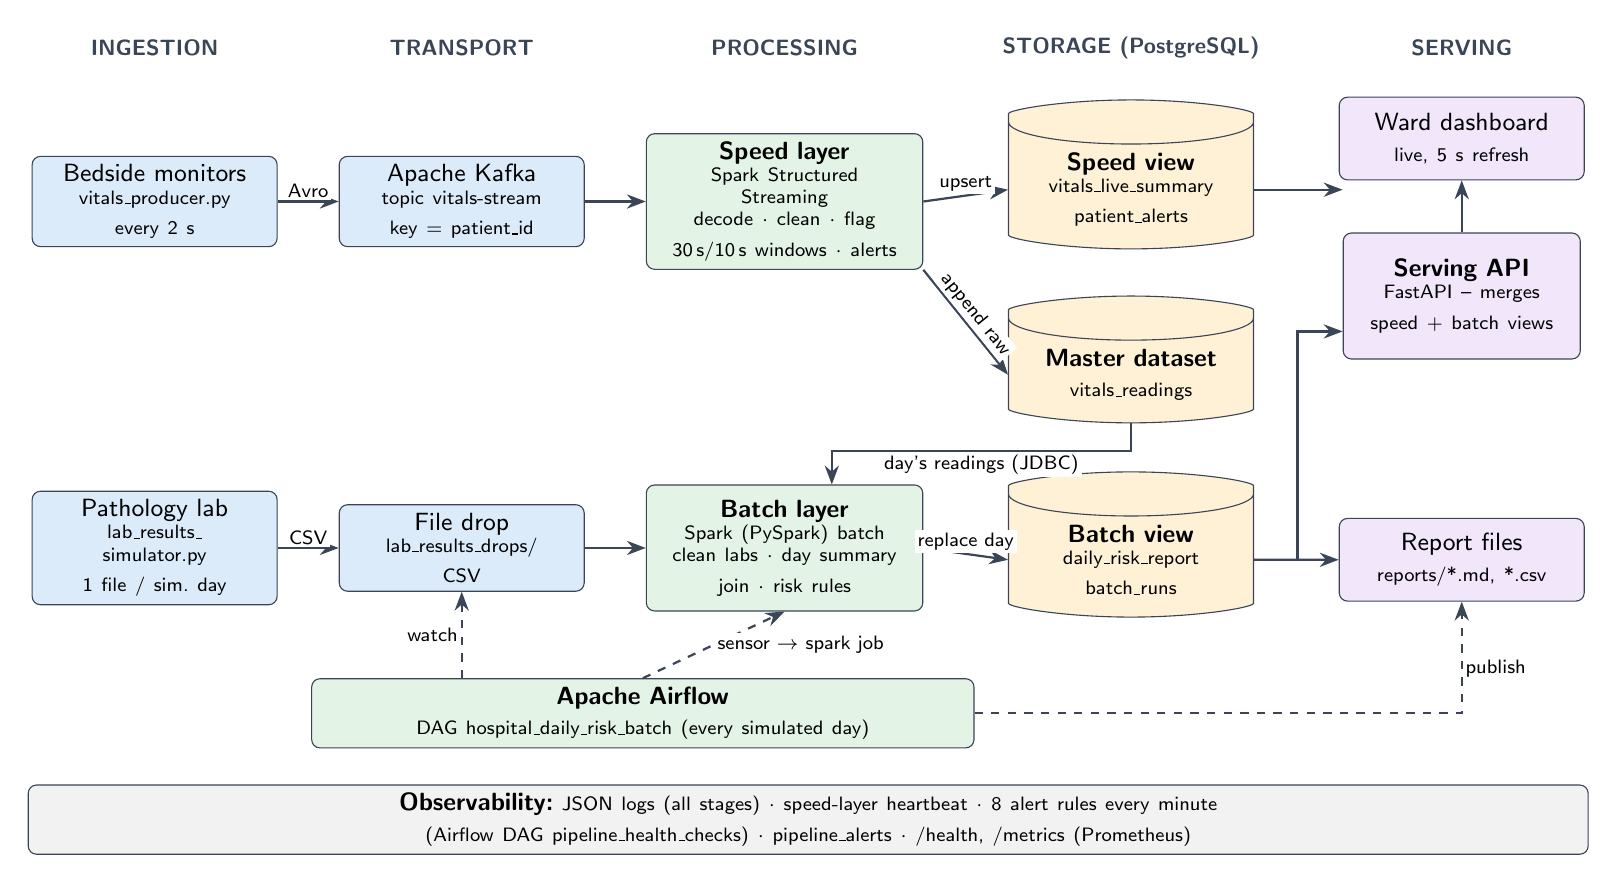
\begin{tikzpicture}[
  font=\sffamily\small,
  box/.style={draw=edge, rounded corners=3pt, align=center, minimum height=1.05cm, text width=2.9cm, inner sep=3pt},
  db/.style={box, cylinder, shape border rotate=90, aspect=0.18, text width=2.9cm, minimum height=1.1cm},
  arr/.style={-{Stealth[length=2.4mm]}, thick, draw=edge},
  lbl/.style={font=\sffamily\scriptsize, fill=white, inner sep=1pt}
]
% Column headers
\foreach \x/\t in {0/INGESTION, 3.9/TRANSPORT, 8.0/PROCESSING, 12.4/STORAGE (PostgreSQL), 16.6/SERVING}
  \node[font=\sffamily\bfseries\footnotesize, text=edge] at (\x, 4.15) {\t};

% Ingestion
\node[box, fill=ingest] (prod) at (0, 2.2) {Bedside monitors\\\scriptsize vitals\_producer.py\\every 2 s};
\node[box, fill=ingest] (lab)  at (0,-2.2) {Pathology lab\\\scriptsize lab\_results\_\\simulator.py\\1 file / sim.\ day};

% Transport
\node[box, fill=ingest] (kafka) at (3.9, 2.2) {Apache Kafka\\\scriptsize topic vitals-stream\\key = patient\_id};
\node[box, fill=ingest] (drop)  at (3.9,-2.2) {File drop\\\scriptsize lab\_results\_drops/\\CSV};

% Processing
\node[box, fill=process, text width=3.3cm, minimum height=1.6cm] (speed) at (8.0, 2.2)
  {\textbf{Speed layer}\\\scriptsize Spark Structured\\Streaming\\decode $\cdot$ clean $\cdot$ flag\\30\,s/10\,s windows $\cdot$ alerts};
\node[box, fill=process, text width=3.3cm, minimum height=1.6cm] (batch) at (8.0,-2.2)
  {\textbf{Batch layer}\\\scriptsize Spark (PySpark) batch\\clean labs $\cdot$ day summary\\join $\cdot$ risk rules};

% Storage
\node[db, fill=store] (master) at (12.4, 0) {\textbf{Master dataset}\\\scriptsize vitals\_readings};
\node[db, fill=store] (live)   at (12.4, 2.35) {\textbf{Speed view}\\\scriptsize vitals\_live\_summary\\patient\_alerts};
\node[db, fill=store] (risk)   at (12.4,-2.35) {\textbf{Batch view}\\\scriptsize daily\_risk\_report\\batch\_runs};

% Serving
\node[box, fill=serve, text width=2.8cm, minimum height=1.6cm] (api) at (16.6, 1.0)
  {\textbf{Serving API}\\\scriptsize FastAPI -- merges\\speed + batch views};
\node[box, fill=serve] (dash) at (16.6, 3.0) {Ward dashboard\\\scriptsize live, 5 s refresh};
\node[box, fill=serve] (files) at (16.6,-2.35) {Report files\\\scriptsize reports/*.md, *.csv};

% Orchestration and observability bands
\node[box, fill=process, text width=8.2cm, minimum height=0.8cm] (airflow) at (6.2,-4.3)
  {\textbf{Apache Airflow}\\\scriptsize DAG hospital\_daily\_risk\_batch (every simulated day)};
\node[box, fill=obs, text width=19.6cm, minimum height=0.8cm] (obsv) at (8.3,-5.65)
  {\textbf{Observability:}\ \scriptsize JSON logs (all stages)\ $\cdot$\ speed-layer heartbeat\ $\cdot$\
   8 alert rules every minute (Airflow DAG pipeline\_health\_checks)\ $\cdot$\ pipeline\_alerts\ $\cdot$\
   /health, /metrics (Prometheus)};

% Flows
\draw[arr] (prod) -- node[lbl, above] {Avro} (kafka);
\draw[arr] (lab) -- node[lbl, above] {CSV} (drop);
\draw[arr] (kafka) -- (speed);
\draw[arr] (drop) -- (batch);
\draw[arr] (speed.east) -- node[lbl, above] {upsert} (live.west);
\draw[arr] (speed.south east) -- node[lbl, pos=0.5, sloped, above] {append raw} (master.west);
\draw[arr] (master.south) -- ++(0,-0.35) -| node[lbl, pos=0.25, below] {day's readings (JDBC)} ($(batch.north)+(0.6,0)$);
\draw[arr] (batch.east) -- node[lbl, above] {replace day} (risk.west);
\draw[arr] (live.east) -- (api.west |- live.east);
\draw[arr] (risk.east) -- ++(0.55,0) |- ($(api.west)+(0,-0.45)$);
\draw[arr] (risk.east) -- (files.west);
\draw[arr] (api.north) -- (dash.south);
\draw[arr, dashed] (airflow.north) -- node[lbl, right] {sensor $\rightarrow$ spark job} ($(batch.south)$);
\draw[arr, dashed] (drop.south |- airflow.north) -- node[lbl, left] {watch} (drop.south);
\draw[arr, dashed] (airflow.east) -| node[lbl, pos=0.7, right] {publish} (files.south);
\end{tikzpicture}}
\caption{Implemented Lambda architecture. Solid arrows are data flow; dashed arrows are
orchestration. The speed layer writes both the raw master dataset and the speed view. The batch
layer recomputes each day from the master dataset.}
\label{fig:arch}
\end{figure}

\subsection{Speed layer (real-time path)}
The speed layer (\code{processing/speed_layer_stream.py}) is one Spark application running two
streaming queries on the same Kafka source (Figure~\ref{fig:speed}):

\begin{itemize}
  \item \textbf{Decode and clean.} Payloads are decoded with \code{from_avro} using Member~A's
  schema file (\code{vitals.avsc}), so there is a single source of truth for the schema. Decoding
  runs in \code{PERMISSIVE} mode, so a corrupt message becomes a rejected row instead of crashing
  the job. Event time comes from the device timestamp, falling back to the broker timestamp.
  Readings are rejected if the patient id is malformed, a value is missing, a value is
  physiologically impossible (e.g.\ HR outside 20--250\,bpm, SpO\textsubscript{2}
  outside 50--100\%), or systolic $\le$ diastolic.
  \item \textbf{Query 1 -- master dataset (append, 5\,s trigger).} Every valid reading is inserted
  into \code{vitals_readings} with primary key \code{(kafka_partition, kafka_offset)} and
  \code{ON CONFLICT DO NOTHING}. With Spark checkpointing this gives an exactly-once
  \emph{effect}: a replay after a crash cannot create duplicates.
  \item \textbf{Query 2 -- speed view (update mode, 10\,s trigger).} Event-time windows of
  30\,s sliding every 10\,s per patient, with a 30\,s watermark, compute average HR, SpO\textsubscript{2}
  and temperature, abnormal count and extremes. Windows are \emph{upserted} into
  \code{vitals_live_summary} on \code{(patient_id, window_start, window_end)}. Each window is
  also classified for a per-patient alert (Section~\ref{sec:rules}). Overlapping breaching
  windows extend one \emph{alert episode} in \code{patient_alerts}, so one spike does not
  produce three alerts.
\end{itemize}

\begin{figure}[!ht]
\centering
\resizebox{0.95\textwidth}{!}{%
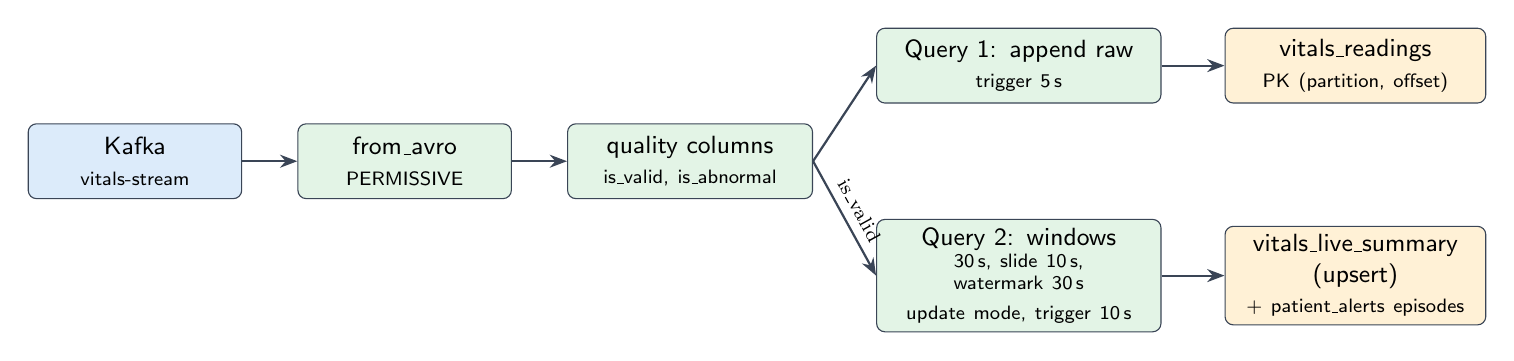
\begin{tikzpicture}[font=\sffamily\small,
  box/.style={draw=edge, rounded corners=3pt, align=center, minimum height=0.95cm, text width=2.5cm, inner sep=3pt},
  arr/.style={-{Stealth[length=2.2mm]}, thick, draw=edge}]
\node[box, fill=ingest] (k) {Kafka\\\scriptsize vitals-stream};
\node[box, fill=process, right=0.7cm of k] (d) {from\_avro\\\scriptsize PERMISSIVE};
\node[box, fill=process, right=0.7cm of d, text width=2.9cm] (q) {quality columns\\\scriptsize is\_valid, is\_abnormal};
\node[box, fill=process, above right=0.25cm and 0.8cm of q, text width=3.4cm] (r) {Query 1: append raw\\\scriptsize trigger 5\,s};
\node[box, fill=process, below right=0.25cm and 0.8cm of q, text width=3.4cm] (w) {Query 2: windows\\\scriptsize 30\,s, slide 10\,s, watermark 30\,s\\update mode, trigger 10\,s};
\node[box, fill=store, right=0.8cm of r, text width=3.1cm] (m) {vitals\_readings\\\scriptsize PK (partition, offset)};
\node[box, fill=store, right=0.8cm of w, text width=3.1cm] (s) {vitals\_live\_summary (upsert)\\\scriptsize + patient\_alerts episodes};
\draw[arr] (k) -- (d); \draw[arr] (d) -- (q);
\draw[arr] (q.east) -- (r.west); \draw[arr] (q.east) -- node[above, sloped, font=\scriptsize] {is\_valid} (w.west);
\draw[arr] (r) -- (m); \draw[arr] (w) -- (s);
\end{tikzpicture}}
\caption{Speed-layer dataflow: two streaming queries share one decoded, cleaned input.}
\label{fig:speed}
\end{figure}

\subsection{Batch layer and orchestration}
The batch layer (\code{processing/batch_layer_daily_report.py}) runs once per lab file. It is
triggered by the Airflow DAG \code{hospital_daily_risk_batch}, scheduled every simulated day
(Figure~\ref{fig:dag}):

\begin{enumerate}
  \item \textbf{\code{wait_for_lab_files}} (\code{PythonSensor}) finds lab files that have no
  successful \code{batch_runs} entry and are older than a 10\,s grace period, which avoids
  reading half-written CSVs. It then applies a \textbf{completeness gate}: a day is only processed
  once the master dataset holds readings past that day's end, for example when the speed layer
  is still replaying Kafka after a restart. The wait is bounded; after one extra simulated day it
  proceeds and the job logs the window as possibly incomplete. Backlogs are handed to a single
  Spark run, oldest file first.
  \item \textbf{\code{run_spark_batch_job}} (\code{BashOperator}) runs the PySpark job, passing
  Airflow's \code{run_id} as a correlation id. The job:
  (a) types, validates and de-duplicates the lab CSV, parses \code{reference_range} with a regular
  expression and flags out-of-range results;
  (b) reads the day's raw readings from \code{vitals_readings} over JDBC (the time range is
  pushed down to PostgreSQL);
  (c) summarises each patient: readings, abnormal ratio, averages, minimum SpO\textsubscript{2},
  maximum HR, and least-squares trends (\code{regr_slope}) of HR and SpO\textsubscript{2} per
  minute;
  (d) \emph{full-outer-joins} the vitals summary with the labs on \code{patient_id}, so patients
  with vitals but no labs, and the reverse, are both reported;
  (e) derives the risk before and after the labs (Section~\ref{sec:rules});
  (f) replaces that file's rows in \code{daily_risk_report} in one transaction, which makes it
  idempotent under Airflow retries, and records the run in \code{batch_runs}.
  \item \textbf{\code{validate_report_output}} checks that the run succeeded and that the stored
  row count matches the count written.
  \item \textbf{\code{publish_report}} writes the consolidated report as Markdown and CSV
  (\code{reports/daily_risk_report_dayN_<epoch>.md/.csv}).
\end{enumerate}

\begin{figure}[!ht]
\centering
\resizebox{0.95\textwidth}{!}{%
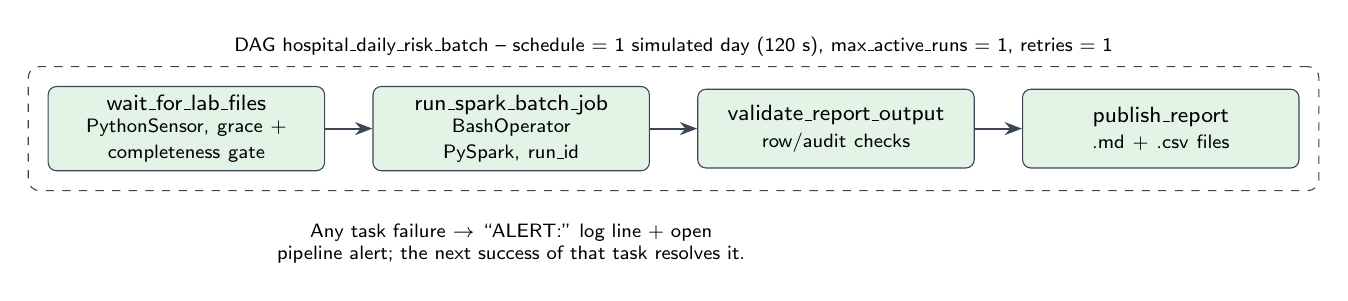
\begin{tikzpicture}[font=\sffamily\small,
  box/.style={draw=edge, rounded corners=3pt, align=center, minimum height=1.0cm, text width=3.3cm, inner sep=3pt, fill=process, font=\sffamily\footnotesize},
  arr/.style={-{Stealth[length=2.2mm]}, thick, draw=edge}]
\node[box] (a) {wait\_for\_lab\_files\\\scriptsize PythonSensor, grace +\\completeness gate};
\node[box, right=0.6cm of a] (b) {run\_spark\_batch\_job\\\scriptsize BashOperator\\PySpark, run\_id};
\node[box, right=0.6cm of b] (c) {validate\_report\_output\\\scriptsize row/audit checks};
\node[box, right=0.6cm of c] (d) {publish\_report\\\scriptsize .md + .csv files};
\draw[arr] (a) -- (b); \draw[arr] (b) -- (c); \draw[arr] (c) -- (d);
\node[draw=edge, dashed, rounded corners, fit=(a)(d), inner sep=7pt, label={[font=\sffamily\scriptsize]above:DAG hospital\_daily\_risk\_batch -- schedule = 1 simulated day (120 s), max\_active\_runs = 1, retries = 1}] {};
\node[below=0.55cm of b, font=\sffamily\scriptsize, text width=10cm, align=center]
  {Any task failure $\rightarrow$ ``ALERT:'' log line + open pipeline alert; the next success of that task resolves it.};
\end{tikzpicture}}
\caption{Airflow DAG for the batch path.}
\label{fig:dag}
\end{figure}

\subsection{Storage and serving layer}
PostgreSQL stores all views (Table~\ref{tab:tables}). The schema script is additive and
idempotent, so it runs safely on the team's existing Supabase database as well as the bundled
container. The FastAPI serving layer (\code{storage/api.py}) \emph{merges} the speed and batch
views. For example, \code{/api/ward/live} returns each patient's latest reading, latest window
and active alert next to the patient's latest daily risk flag.

\begin{table}[!ht]
\centering\small
\begin{tabularx}{\textwidth}{@{}P{4.0cm}P{2.6cm}L@{}}
\toprule
\textbf{Table} & \textbf{Written by} & \textbf{Purpose / key design point} \\
\midrule
\code{vitals_readings} & speed layer (Q1) & Master dataset; PK \code{(kafka_partition, kafka_offset)} makes replay idempotent. \\
\code{vitals_live_summary} & speed layer (Q2) & Speed view; unique \code{(patient_id, window_start, window_end)} for upserts. \\
\code{patient_alerts} & speed layer (Q2) & Per-patient alert episodes (severity, reasons, extremes, window span). \\
\code{daily_risk_report} & batch layer & Batch view; one row per (patient, lab test), keyed by source file. \\
\code{batch_runs} & batch layer & Audit trail: run id, file, status, rows, patients, duration, error. \\
\code{pipeline_heartbeat} & speed-layer driver & Liveness, per-query progress and counters. \\
\code{pipeline_alerts} & health checks, Airflow & Pipeline alert lifecycle (open $\rightarrow$ resolved). \\
\bottomrule
\end{tabularx}
\caption{Storage model.}
\label{tab:tables}
\end{table}

\begin{table}[!ht]
\centering\small
\begin{tabularx}{\textwidth}{@{}P{5.6cm}L@{}}
\toprule
\textbf{Endpoint} & \textbf{Returns} \\
\midrule
\code{GET /api/ward/live} & Real-time ward figures (active patients, readings and abnormal ratio in the last 5 min, ward averages) and per-patient status. \\
\code{GET /api/patients/{id}} & Recent readings, windows, alerts and the latest daily risk for one patient. \\
\code{GET /api/alerts} & Per-patient threshold alert episodes. \\
\code{GET /api/reports/daily[/latest]} & The consolidated daily risk report(s). \\
\code{GET /api/pipeline/alerts}, \code{/health}, \code{/metrics} & Observability (Section~\ref{sec:obs}). \\
\code{GET /} & Live ward dashboard (HTML, polls the API every 5\,s). \\
\bottomrule
\end{tabularx}
\caption{Serving API.}
\end{table}

% =============================================================================
\section{Processing Rules}\label{sec:rules}
% =============================================================================
Thresholds are the same ones the producer uses to label its readings, so ingestion and
processing agree:

\begin{itemize}
  \item \textbf{Abnormal reading:} HR $<60$ or $>100$\,bpm, or SpO\textsubscript{2} $<95\%$, or
  temperature $>37.5\,^\circ$C.
  \item \textbf{Per-patient alert (per window).} \emph{Critical} if the window average
  SpO\textsubscript{2} is below 90\%, HR is below 50 or above 130\,bpm, or temperature is at
  least 39\,$^\circ$C. Otherwise \emph{warning} if the window contains any abnormal reading.
  \item \textbf{Concerning vitals (daily).} For a patient with $n>0$ readings, of which $a$ are
  abnormal:
  \[
    \text{concerning} \iff \frac{a}{n} \ge 0.20 \;\lor\; \overline{HR}\notin[60,100] \;\lor\;
    \overline{SpO_2} < 95 \;\lor\; \overline{T} > 37.5
  \]
  \item \textbf{Abnormal lab:} the result lies outside the reference range parsed from the file.
  \item \textbf{Risk flag:} \code{high} (concerning vitals \emph{and} abnormal labs),
  \code{elevated_vitals}, \code{elevated_labs} (vitals looked normal; the labs changed the
  picture) or \code{normal}. The report also stores \code{vitals_only_risk},
  \code{risk_changed_by_labs} and a human-readable \code{risk_reasons}. It lists which patients
  were \emph{escalated} by the labs and which were \emph{newly flagged} by them. These two lists
  answer the second half of the business question directly.
\end{itemize}

% =============================================================================
\section{Technology Stack and Justification}
% =============================================================================
Table~\ref{tab:stack} justifies each major component against a specific constraint of the
ward-monitoring scenario, rather than general popularity.
\begin{table}[!ht]
\centering\small
\begin{tabularx}{\textwidth}{@{}P{2.3cm}P{2.9cm}L@{}}
\toprule
\textbf{Layer} & \textbf{Choice} & \textbf{Justification tied to the use case} \\
\midrule
Ingestion & Apache Kafka (Confluent Cloud) with Avro &
Bedside data must not be lost when a consumer is down. Kafka's durable, replayable log let the
speed layer catch up after our outage test with no gap. Keying by \code{patient_id} keeps each
patient's readings in order within a partition. Avro gives a compact, typed contract shared by
the producer and Spark. A managed cluster avoided running brokers on student laptops. \\
Stream processing & Spark Structured Streaming &
Needs event-time windows and watermarks for out-of-order sensor data, checkpointed recovery, and
foreachBatch sinks for idempotent upserts. We chose it over Apache Storm because the same engine
and DataFrame API also runs the batch layer, so the rules are shared and one skill set suffices.
It also runs on Databricks, where the team first prototyped it. \\
Batch processing & Spark (PySpark) &
Same code style and rule module as the stream. JDBC range push-down reads only one day. It scales
out without a rewrite if more wards are added. \\
Orchestration & Apache Airflow &
The daily feed needs a file sensor, ordered dependencies (sensor $\rightarrow$ Spark
$\rightarrow$ validate $\rightarrow$ publish), retries and failure callbacks, plus a visible run
history. Airflow also schedules the minute-by-minute health checks. \\
Storage & PostgreSQL (Supabase / local) &
The data is small, relational and joined constantly (patients, windows, alerts, reports).
\code{ON CONFLICT} upserts give idempotency for stream replays and batch retries, and one SQL
store serves both views to the API. We preferred it to Cassandra, whose partition-oriented model
suits write-heavy scale but makes the ad-hoc joins and aggregates of the serving layer awkward. \\
Serving & FastAPI + HTML dashboard &
Lightweight JSON API matching the suggested ``API endpoint for real-time ward monitoring
figures'', with auto-generated OpenAPI docs and a Prometheus \code{/metrics} export. \\
Deployment & Docker Compose &
One command starts PostgreSQL, the schema migration, the speed layer, the API, Airflow and
optional Prometheus from a single image (Airflow + Java 17 + PySpark 3.5), giving reproducible
demos. \\
\bottomrule
\end{tabularx}
\caption{Technology stack.}\label{tab:stack}
\end{table}

% =============================================================================
\section{Observability Design}\label{sec:obs}
% =============================================================================
The goal is to \emph{detect} a failure and \emph{diagnose which stage} failed, not just to know
that something is wrong.

\subsection{Structured logging (all stages)}
Every component logs one JSON object per line, with the same core keys as the ingestion scripts
(\code{timestamp, level, component, message}) plus structured fields. Airflow's \code{run_id}
is passed into the Spark job and stored in \code{batch_runs} and \code{daily_risk_report}, so one
run can be traced from the DAG through Spark to the stored rows. Alert lines start with the
marker \code{ALERT:}. An example from the speed layer:

\begin{lstlisting}
{"timestamp": "2026-09-29T17:37:31.519+00:00", "level": "CRITICAL",
 "component": "speed_layer",
 "message": "ALERT: patient P104 critical - SpO2 89.9% < 90%; HR 160 bpm > 130; ...",
 "alert_type": "patient_vitals", "alert_id": 18, "patient_id": "P104",
 "severity": "critical"}
\end{lstlisting}

Other log events include: rows in, written and rejected per micro-batch (with samples of rejected
records); window upserts and alert counts; a heartbeat with Spark query progress (input rows/s,
trigger duration, watermark, state rows); per-run batch statistics; and one access-log line per
API request.

\subsection{Metrics}
One module (\code{observability/metrics.py}) computes the metrics, which feed the rule engine,
\code{/health} and the Prometheus \code{/metrics} export, so the numbers can never disagree.
Table~\ref{tab:metrics} lists the metrics per stage.

\begin{table}[!ht]
\centering\small
\begin{tabularx}{\textwidth}{@{}P{2.4cm}L@{}}
\toprule
\textbf{Stage} & \textbf{Metrics (Prometheus gauges, prefix \code{hospital_})} \\
\midrule
Ingestion & age of newest stored reading; end-to-end event$\rightarrow$storage lag; readings and abnormal ratio (5 min); active patients (2 min); age of newest lab file \\
Processing & speed-layer heartbeat age; Kafka input rows/s; reject ratio; speed-view freshness; batch successes/failures (30 min); failure ratio; last success age; last duration; pending lab files \\
Storage/serving & database up; active and 24\,h patient alerts; open pipeline alerts; \code{health_rule_breached{rule=...}} \\
\bottomrule
\end{tabularx}
\caption{Exported metrics.}
\label{tab:metrics}
\end{table}

\subsection{Alert and health-check rules}
Rules are stored as data (\code{observability/alert_rules.json}). The Airflow DAG
\code{pipeline_health_checks} evaluates them every minute, and \code{observability/prometheus/alert_rules.yml}
mirrors them for Prometheus. Each rule has a lifecycle: a new breach opens a
\code{pipeline_alerts} row and logs \code{ALERT:}; a continuing breach only updates the row (no
log spam); recovery marks the row \emph{resolved} and logs \code{RESOLVED:}. While any critical
rule is breached, the health task fails, so Airflow's grid view doubles as a health history.

\begin{table}[!ht]
\centering\small
\begin{tabularx}{\textwidth}{@{}P{4.4cm}P{3.5cm}P{1.3cm}L@{}}
\toprule
\textbf{Rule} & \textbf{Condition} & \textbf{Severity} & \textbf{Diagnoses} \\
\midrule
\code{vitals_stream_stale} & no reading stored for 60\,s & critical & producer, Kafka or speed layer down \\
\code{speed_layer_down} & no heartbeat for 60\,s & critical & Spark job crashed (vs.\ producer silent) \\
\code{live_summary_stale} & no window update for 90\,s & warning & aggregation query stuck \\
\code{lab_feed_stale} & no lab file for 2.5 sim.\ days & warning & daily source late \\
\code{batch_backlog} & $>2$ lab files waiting & warning & Airflow or batch falling behind \\
\code{batch_job_failing} & $>20\%$ runs failed (30 min) & critical & batch job broken \\
\code{data_quality_rejects_high} & $>5\%$ readings rejected & warning & producer or schema problem \\
\code{ward_abnormal_rate_high} & $>30\%$ abnormal (5 min) & warning & ward-wide event or faulty sensors \\
\bottomrule
\end{tabularx}
\caption{Pipeline alert rules. In addition, any failed Airflow task raises an alert that the
task's next success resolves.}
\end{table}

\textbf{Why these signals.} Pairing \emph{data freshness} (newest stored reading) with
\emph{process liveness} (the heartbeat) separates ``the producer or Kafka is silent'' from ``the
Spark job died''. The reject ratio separates data-quality problems from outages. The batch
backlog and failure ratio localise problems to the daily path.

% =============================================================================
\section{Results}
% =============================================================================
\textbf{Test setup.} The results below come from an end-to-end run of the Docker Compose stack
(speed layer, Airflow, PostgreSQL, API, Prometheus) together with Member~A's own reading
generator and lab simulator (120\,s simulated day). For the recorded run, the producer published
to a local single-broker Kafka instead of the shared Confluent Cloud cluster, and at a faster
rate (one reading per second). One message in 25 was deliberately corrupted to exercise the
data-quality path. This is why the dashboard shows a \code{data_quality_rejects_high} warning
(reject ratio about 6\%). Nine simulated days were processed.

\subsection{Live ward dashboard (speed + batch views)}
Figure~\ref{fig:dashboard} shows the dashboard at \code{http://localhost:8000}:
\begin{itemize}
  \item \textbf{Top:} real-time ward figures (15 active patients, 295 readings and a 7\% abnormal
  rate in the last 5 minutes, 4 patients in critical state).
  \item \textbf{Middle:} per-patient latest vitals, the current 30\,s window, active alerts and
  each patient's latest daily risk flag, with recent patient-alert episodes and open pipeline
  alerts alongside.
  \item \textbf{Bottom:} the latest consolidated daily risk report.
\end{itemize}

\begin{figure}[!ht]
\centering
\screenshot{figures/dashboard.png}{\textwidth}{live ward dashboard}
\caption{Live ward dashboard served by the FastAPI serving layer.}
\label{fig:dashboard}
\end{figure}

\subsection{Consolidated daily risk report}
Table~\ref{tab:report} is an extract of the report generated for simulated day~3 (file
\code{reports/daily_risk_report_day3_1790703438.md}), with 120 readings in the vitals window.
Of the 15 patients: 1 \emph{high}, 2 \emph{elevated\_vitals}, 2 \emph{elevated\_labs},
10 \emph{normal}. The report states directly how the labs changed the picture: \textbf{P104}
was escalated from \emph{elevated} to \emph{high} (low average SpO\textsubscript{2} confirmed
by an abnormal CRP), and \textbf{P100} and \textbf{P101} were \emph{newly flagged by labs alone}
although their vitals looked normal.

\begin{table}[!ht]
\centering\footnotesize
\begin{tabularx}{\textwidth}{@{}lllrrrrL@{}}
\toprule
\textbf{Patient} & \textbf{Risk} & \textbf{Vitals-only} & \textbf{Read.} & \textbf{Abn.\%} & \textbf{Avg HR} & \textbf{Avg SpO\textsubscript{2}} & \textbf{Reasons} \\
\midrule
P104 & high & elevated & 6 & 17 & 75 & 94.9 & avg SpO\textsubscript{2} 94.9\%; abnormal labs: CRP \\
P106 & elevated\_vitals & elevated & 6 & 17 & 87 & 94.7 & avg SpO\textsubscript{2} 94.7\% \\
P113 & elevated\_vitals & elevated & 12 & 25 & 77 & 93.8 & 25\% of 12 readings abnormal; avg SpO\textsubscript{2} 93.8\% \\
P100 & elevated\_labs & normal & 10 & 0 & 75 & 97.9 & abnormal labs: Glucose \\
P101 & elevated\_labs & normal & 8 & 0 & 81 & 96.8 & abnormal labs: Hemoglobin \\
P102 & normal & normal & 12 & 0 & 77 & 97.2 & -- \\
\multicolumn{8}{@{}l}{\itshape \dots\ 9 further patients classified normal} \\
\bottomrule
\end{tabularx}
\caption{Extract of the consolidated daily risk report for simulated day 3.}
\label{tab:report}
\end{table}

\subsection{Batch layer and orchestration}
Every simulated day, Airflow detected the new lab file, ran the Spark batch job, validated the
output and published the report files without manual action. Table~\ref{tab:batch} shows the
first three runs as recorded in \code{batch_runs}. A Spark batch run takes about 6--7.5\,s,
including JVM start-up, which is far below the 120\,s budget of a simulated day.

\begin{table}[!ht]
\centering\small
\begin{tabular}{@{}lrrrr@{}}
\toprule
\textbf{Lab file (simulated day)} & \textbf{Report rows} & \textbf{Patients} & \textbf{High risk} & \textbf{Spark run (s)} \\
\midrule
\code{lab_results_day1_1790703198.csv} & 10 & 5 & 0 & 6.0 \\
\code{lab_results_day2_1790703318.csv} & 12 & 6 & 0 & 7.4 \\
\code{lab_results_day3_1790703438.csv} & 27 & 15 & 1 & 7.3 \\
\bottomrule
\end{tabular}
\caption{First batch-layer runs.}
\label{tab:batch}
\end{table}

\begin{figure}[!ht]
\centering
\screenshot{figures/airflow_dags.png}{0.95\textwidth}{Airflow UI -- grid view of the DAGs
\texttt{hospital\_daily\_risk\_batch} and \texttt{pipeline\_health\_checks}}
\caption{Airflow orchestrating the daily batch path and the minute-by-minute health checks.}
\end{figure}

\subsection{Failure drill: detection, diagnosis and recovery}
To test observability and the Lambda recovery properties, we stopped the speed layer
(\code{docker compose stop speed-layer}) at 17:39:25 and restarted it about two minutes later.

\begin{table}[!ht]
\centering\small
\begin{tabularx}{\textwidth}{@{}P{1.9cm}L@{}}
\toprule
\textbf{Time (UTC)} & \textbf{Observed behaviour} \\
\midrule
17:39:25 & Speed layer stopped; the producer keeps publishing to Kafka. \\
17:41:01 & Health DAG opens \code{vitals_stream_stale} (critical), \code{speed_layer_down} (critical)
and \code{live_summary_stale} (warning). \code{ALERT:} lines are logged, the health task fails
(red in Airflow), the dashboard shows \code{health: critical}. The heartbeat rule identifies the
Spark job, not the producer, as the cause. \\
$\approx$17:41:35 & Speed layer restarted; it resumes from its checkpoint and replays the missed Kafka offsets. \\
17:41:51 & \code{vitals_stream_stale} and \code{live_summary_stale} resolved. \\
17:43:01 & \code{speed_layer_down} resolved (first heartbeats observed). \\
\bottomrule
\end{tabularx}
\caption{Failure-drill timeline.}
\end{table}

\textbf{No data loss.} Counting stored readings per minute across the outage gives 58, 49,
\textbf{67, 60, 57}, 58 for 17:37--17:42. The outage minutes are complete. Their readings were
stored up to 2\,min\,38\,s late, during the replay, instead of being lost. Normal end-to-end lag
from event to storage was about 6--18\,s. The only Kafka offsets missing from
\code{vitals_readings} are the deliberately corrupted messages, which were rejected and counted.

\begin{figure}[!ht]
\centering
\screenshot{figures/failure_drill_alerts.png}{0.95\textwidth}{\texttt{pipeline\_health\_checks}
task log (or dashboard) showing the \texttt{ALERT:} lines during the outage}
\caption{Alerts raised while the speed layer was stopped.}
\end{figure}

\subsection{Batch recomputation (``batch corrects speed'')}\label{sec:recompute}
The run also exposed a real completeness problem, and showed Lambda correcting it. Days~1 and~2
were computed while the speed layer was still starting up and replaying Kafka. Their reports
therefore contained \textbf{0} readings, although the master dataset later held \textbf{33} and
\textbf{115} readings for those windows. Two changes followed:
\begin{enumerate}
  \item We re-ran the idempotent batch job for the two files (one \code{--lab-file} argument
  each). The rows for those days were replaced with
  the correct counts (33 and 115) and the other days were untouched.
  \item We added the \textbf{completeness gate} described in Section~3.3, so the DAG now waits for
  the master dataset to cover a day before processing it. All later days matched the master
  dataset exactly (e.g.\ day~4: 106 of 106 readings; day~5: 128 of 128).
\end{enumerate}

\subsection{Automated tests}
18 automated tests pass (\code{pytest}), inside the Docker image with PySpark and Java~17. They
cover:
\begin{itemize}
  \item lab-file discovery, including restarts of the simulator and the completeness gate;
  \item the clinical and alert rules, the health-rule engine, the Prometheus export and JSON
  logging;
  \item Spark transformations, including decoding real Avro payloads produced the same way as the
  producer (corrupt, impossible and bad-timestamp messages), sliding-window counts, lab cleaning
  and de-duplication, and the risk matrix.
\end{itemize}

% =============================================================================
\section{Limitations, Trade-offs and Production-Scale Changes}
% =============================================================================
\subsection{Limitations and trade-offs}
\begin{itemize}
  \item \textbf{Two code paths (Lambda's cost).} The speed and batch layers must implement the
  same rules. This is mitigated by shared rule and threshold modules and tests, but not eliminated.
  \item \textbf{Sparse simulation.} 15 patients and one reading every 2\,s give about one reading
  per patient per 30\,s window and about 8 readings per patient per simulated day. Window
  averages are often a single reading, and the per-day trend slopes are noisy. The trends are
  reported but deliberately not used in the risk rule.
  \item \textbf{Driver-side writes.} Micro-batches are collected to the Spark driver and written
  with \code{psycopg2}. This is fine for one ward, but a bottleneck at scale.
  \item \textbf{PostgreSQL as master dataset.} It is simple and transactional but grows without
  bound. There is no partitioning or retention policy.
  \item \textbf{Batch runs locally, not on Databricks.} Databricks Community Edition has no Jobs
  REST API, so Airflow cannot trigger it. It also cannot read the lab files, which live on the
  simulator's machine. The Spark code is Databricks-compatible, but the batch job is run as local
  PySpark from Airflow.
  \item \textbf{Secrets.} Credentials come from a git-ignored \code{.env} file or a Databricks
  secret scope. Community Edition cannot create secret scopes, so notebook runs need credentials
  in a cell that must be cleared before export.
  \item \textbf{Alerting stops at logs, database and dashboard.} There is no paging integration
  (e.g.\ email, Slack, PagerDuty). Clinical thresholds are simplified population ranges, not
  patient-specific baselines or a validated score such as NEWS2.
  \item \textbf{Single-node components.} The demo runs Spark \code{local[2]}, Airflow's
  LocalExecutor and a single PostgreSQL instance.
\end{itemize}

\subsection{What we would do differently at production scale}
\begin{itemize}
  \item Store the master dataset in a lakehouse table (Delta Lake or Apache Iceberg on object
  storage) partitioned by date. Keep PostgreSQL only for the small serving views, or move them
  to a low-latency store.
  \item Use distributed \code{foreachPartition} writers or native connectors instead of
  driver-side writes. Run Spark on a managed cluster (Databricks Jobs or EMR), triggered through
  the Airflow Databricks provider.
  \item Enforce data contracts with a schema registry (Confluent Schema Registry) and a
  dead-letter topic for rejected messages. Right-size Kafka partitions and retention per ward.
  \item Run Airflow with a Celery or Kubernetes executor, managed secrets (e.g.\ Vault or a cloud
  secret manager), and Grafana dashboards with Alertmanager routing to on-call staff.
  \item Replace the fixed thresholds with clinically validated early-warning scores and
  per-patient baselines, and add access control and audit logging for patient data (HIPAA- or
  GDPR-style compliance).
  \item Evaluate a Kappa-style unification once the platform runs on a lakehouse with streaming
  tables. Its main drawback here, reprocessing through long log retention, largely disappears when
  the master dataset is itself a replayable table.
\end{itemize}

% =============================================================================
\section{Conclusion}
% =============================================================================
We built a complete Lambda pipeline for ward vital-sign monitoring. Kafka ingests bedside
readings. A Spark Structured Streaming speed layer serves live ward figures and per-patient
alerts within seconds, and also persists an immutable master dataset. An Airflow-orchestrated
Spark batch layer recomputes each simulated day and joins it with the pathology lab's daily
file. The resulting consolidated risk report shows, per patient, how the latest lab results
escalate or newly raise the risk. The system is observable end to end: structured logs,
correlated run ids, a heartbeat, exported metrics, and eight alert rules. In an outage test these
detected and localised a failure within about a minute and a half, and the system then recovered
with no data loss. The same test showed the main benefit of the chosen architecture: a day
computed from incomplete data was corrected simply by re-running the batch layer.

% =============================================================================
\appendix
\section{Individual Contributions}
% =============================================================================
\begin{table}[!ht]
\centering\small
\begin{tabularx}{\textwidth}{@{}P{3.6cm}L@{}}
\toprule
\textbf{Member} & \textbf{Contribution} \\
\midrule
Arachchi W.A.T.T.W\newline EG/2021/4412\newline (Member A -- Ingestion) &
Streaming vitals simulator with Avro serialisation and abnormal-spike generation
(\code{vitals_producer.py}, \code{vitals.avsc}); daily lab-results simulator
(\code{lab_results_simulator.py}); Confluent Cloud cluster and topic set-up; structured logging
for ingestion; Kafka--Databricks connectivity (the \code{kafkashaded.} JAAS fix). \\
Akurana B.N.T.M\newline EG/2020/3812\newline (Member B -- Processing) &
Spark Structured Streaming speed layer (Avro decoding, cleaning, abnormal flagging, sliding-window
aggregation, master-dataset and speed-view sinks, per-patient alert episodes); Spark batch layer
(lab cleaning, day recomputation from the master dataset, vitals--lab join, risk rules);
Databricks prototyping; transformation tests. \\
Nadha M.J\newline EG/2021/4686\newline (Member C -- Orchestration, storage \& observability) &
PostgreSQL schema and migrations; FastAPI serving layer and live dashboard; Airflow DAGs (daily
batch with completeness gate, health checks, failure callbacks); observability (metrics module,
alert-rule engine, alert lifecycle, Prometheus export and rules); Docker Compose deployment;
end-to-end and failure-drill testing. \\
\bottomrule
\end{tabularx}
\end{table}

\section{Reproducing the Results}
\begin{lstlisting}
cp .env.example .env          # add Confluent Cloud BOOTSTRAP_SERVER / API_KEY / API_SECRET
docker compose build
docker compose up -d          # add --profile monitoring for Prometheus (:9090)
python vitals_producer.py     # terminal 1 (repository root)
python lab_results_simulator.py   # terminal 2 (repository root)
# Dashboard http://localhost:8000   API docs /docs   Airflow http://localhost:8080 (admin/admin)
docker compose run --rm --no-deps --entrypoint python api -m pytest -q   # tests
\end{lstlisting}

\textbf{Assumptions and simplifications.} One simulated day is 120\,s. There is a fixed pool of 15
patients. Timestamps are stored in UTC. The lab file for a simulated day covers the vitals of the
120\,s preceding its drop time. Clinical thresholds are simplified adult reference ranges.

\end{document}
